\documentclass[a4paper]{article}
\usepackage[UTF8]{ctex}
\usepackage[a4paper,margin=1in]{geometry}
\usepackage{graphicx}
\usepackage{float}
\usepackage{listings}
\usepackage{booktabs}
\usepackage{hyperref}
\usepackage{fancyhdr}
\usepackage{lastpage}
\usepackage{color}
\usepackage{xcolor}
\usepackage{indentfirst}
\setlength{\parindent}{2em}
\usepackage{zhnumber}
\usepackage[dvipsnames]{xcolor}
\usepackage{amsmath}
\usepackage{tikz}
\usetikzlibrary{shapes,arrows,positioning}

% ===== 个人信息与实验信息配置 =====
\newcommand{\projname}{ROSE——编译原理逆向工程工具}
\newcommand{\reporttitle}{实验三-设计文档}
\newcommand{\stuno}{23336179}
\newcommand{\authorname}{马福泉}
\newcommand{\major}{计算机科学与技术}
\newcommand{\adviser}{李文军}
\newcommand{\startdate}{2026年6月}
\newcommand{\labenddate}{2026年6月}
\newcommand{\labroom}{B203}

% ===== 页眉页脚设置 =====
\pagestyle{fancy}
\fancyhf{}
\fancyhead[L]{\kaishu \projname}
\fancyhead[C]{\kaishu \reporttitle}
\fancyhead[R]{\kaishu \authorname}
\fancyfoot[C]{第 \thepage 页，共 \pageref{LastPage} 页}
\renewcommand{\headrulewidth}{0.4pt}
\renewcommand{\footrulewidth}{0pt}

% ===== 代码高亮配置 =====
\definecolor{NavyBlue}{RGB}{0,0,128}
\definecolor{codegreen}{RGB}{0,128,0}
\definecolor{codegray}{RGB}{128,128,128}
\definecolor{codepurple}{RGB}{128,0,128}
\definecolor{backcolour}{RGB}{245,245,245}

\lstset{
    language=Java,
    basicstyle=\ttfamily\small,
    commentstyle=\color{codegreen}\itshape,
    keywordstyle=\color{NavyBlue}\bfseries,
    stringstyle=\color{codepurple},
    numberstyle=\tiny\color{codegray},
    backgroundcolor=\color{backcolour},
    breaklines=true,
    frame=single,
    numbers=left,
    tabsize=4,
    showstringspaces=false,
    captionpos=b,
    escapeinside={\%}{\%},
    morekeywords={enum,record}
}

\begin{document}

% ==================== 封面 ====================
\begin{titlepage}
    \centering
    
    
\includegraphics[width=10cm]{img/SYSULogo.png}

    \vspace{1em}
    {\Large \kaishu \projname \par}
    \vspace{3em}

    {\fontsize{36pt}{40pt}\kaishu \selectfont \boldmath \reporttitle\par}
    \vspace{2em}
    \vspace*{\fill}

    \begin{center}
    {\Large
    \makebox[5em][s]{学号}:\underline{\makebox[15em][c]{\kaishu \stuno}}\\[1em]
    \makebox[5em][s]{姓名}:\underline{\makebox[15em][c]{\kaishu \authorname}}\\[1em]
    \makebox[5em][s]{专业}:\underline{\makebox[15em][c]{\kaishu \major}}\\[1em]
    \makebox[5em][s]{指导教师}:\underline{\makebox[15em][c]{\kaishu \adviser}}\\[1em]
    \makebox[5em][s]{起始日期}:\underline{\makebox[15em][c]{\kaishu \startdate}}\\[1em]
    \makebox[5em][s]{结束日期}:\underline{\makebox[15em][c]{\kaishu \labenddate}}\\[1em]
    \makebox[5em][s]{实验地点}:\underline{\makebox[15em][c]{\kaishu \labroom}}
    }
    \end{center}

    \vspace*{\fill}
\end{titlepage}

% ==================== 目录 ====================
\tableofcontents
\newpage

% ==================== 正文 ====================

\section{实验简述}

本项目 ROSE 是一个编译原理逆向工程工具，旨在对 Oberon-0 语言源程序进行词法分析、语法分析、
语义分析，并自动生成流程图和调用关系图。本实验为第三阶段——使用 JavaCUP 工具自动生成
LALR(1) 语法分析器，实现对 Oberon-0 源程序的语法结构解析，并结合 ROSE 工具集的
CallGraph 库生成过程调用图。

字层（实验二）将字符流转化为 Token 流，语法分析层将 Token 流转化为结构化的语法树，并在此
之上执行语义动作——收集过程声明与调用关系，最终以可视化形式呈现调用依赖图。本实验的核心
挑战在于：(1) 将 Oberon-0 的 EBNF 语法等价转换为 JavaCUP 的声明式产生式规范；
(2) 处理 Token 类型码与 JavaCUP 自动编号间的映射不一致问题；(3) 消除 LALR 分析表中的
歧义冲突；(4) 在语义动作中集成 CallGraph 的过程-调用边收集逻辑。

\section{Oberon-0 语法规则回顾}

Oberon-0 的完整 EBNF 语法定义（摘自 Wirth, 1996）如下。其中 \texttt{Module} 为顶层结构，
包含声明序列（CONST、TYPE、VAR、过程声明）和语句序列。表达式采用经典的运算符优先级分层。
\texttt{Designator}（设计子）的选择器是 Oberon 语言族的特色——通过 \texttt{.字段名} 和
\texttt{[下标]} 实现对 RECORD 和 ARRAY 类型的选择访问。

{\small
\begin{verbatim}
Module     = MODULE ident ";" [ImportList] DeclarationSequence
             [BEGIN StatementSequence] END ident "." .

DeclarationSequence = { CONST {ConstDeclaration ";"} |
                        TYPE {TypeDeclaration ";"}  |
                        VAR  {VarDeclaration ";"} }
                        {ProcedureDeclaration ";" | ForwardDeclaration ";"} .

ConstDeclaration = ident "=" ConstExpression .
TypeDeclaration  = ident "=" Type .
Type             = ident | ARRAY ConstExpression OF Type |
                   RECORD FieldListSequence END .
VarDeclaration   = IdentList ":" Type .
ProcedureDeclaration = PROCEDURE ident [FormalParameters] ";"
                       DeclarationSequence [BEGIN StatementSequence] END ident .
FormalParameters = "(" [FPSection {";" FPSection}] ")" .
FPSection        = [VAR] ident {"," ident} ":" Type .
IdentList        = ident {"," ident} .

StatementSequence = Statement {";" Statement} .
Statement         = [ ident Selector {"," ident Selector} ":=" Expression |
                       ident ["(" [Expression {"," Expression}] ")"] |
                       IF Expression THEN StatementSequence
                            {ELSIF Expression THEN StatementSequence}
                            [ELSE StatementSequence] END |
                       WHILE Expression DO StatementSequence END |
                       Read | Write | WriteLn ] .

Expression        = SimpleExpression [Relation SimpleExpression] .
SimpleExpression  = ["+"|"-"] Term {AddOperator Term} .
Term              = Factor {MulOperator Factor} .
AddOperator       = "+" | "-" | OR .
MulOperator       = "*" | DIV | MOD | "&" .
Factor            = Number | BoolLit | Designator |
                    "(" Expression ")" | "~" Factor .
Designator        = qualident {"." ident | "[" Expression "]"} .
Relation          = "=" | "#" | "<" | "<=" | ">" | ">=" .
\end{verbatim}
}

\section{JavaCUP 文法规范设计}

\subsection{终结符声明}

JavaCUP 要求以 \texttt{terminal} 关键字显式声明所有终结符及其类型。本实验声明了 49 个
终结符，涵盖 16 个保留字（MODULE, BEGIN, END, IF, THEN, ELSIF, ELSE, WHILE, DO,
PROCEDURE, VAR, CONST, TYPE, RECORD, ARRAY, OF）、5 个预定义关键字（INTEGER\_TYPE,
BOOLEAN\_TYPE, Read, Write, WriteLn）、3 种带类型的字面量终结符（Integer INTEGER,
Boolean BOOL\_LIT, String IDENT）、15 个运算符和 10 个分界符。

JavaCUP 按声明顺序为每个终结符自动分配整数编码（从 2 开始，0 为 EOF，1 为 error）。由于
TokTen.java 中使用的常量编号与 JavaCUP 自动分配的编号不一致，需在 CupScanner 桥接器中
通过 HashMap 建立双向映射（49 对）。

\subsection{非终结符声明}

JavaCUP 要求以 \texttt{non terminal} 关键字显式声明所有非终结符及其语义值类型。本实验
声明了 35 个非终结符，其中 \texttt{module} 为起始符号。表达式类非终结符（expr、simple\_expr、
term、factor、designator）的语义值类型为 Object（运行时为 String），标识符列表类的类型为
String。

\subsection{优先级与结合性}

运算符优先级从低到高声明为：\texttt{OR < AND < NOT < 关系(<, <=, =, \#, >, >=)
< +, - < *, DIV, MOD < DOT, LBRACK}。一元加减在 simple\_expr 中直接归约，无需虚终结符。
\texttt{LBRACK} 和 \texttt{DOT} 的优先级声明保证了选择器（\texttt{[expr]} 和
\texttt{.id}）的高紧密度绑定。

\subsection{关键产生式设计}

\textbf{模块结构}：\texttt{module ::= MODULE IDENT ";" decl\_seq BEGIN statement\_seq
END IDENT "."}。顶层语法分析成功后在语义动作中输出过程数与调用图统计信息。

\textbf{声明序列}：\texttt{decl\_seq} 采用左递归结构，每类声明（CONST、TYPE、VAR、
PROCEDURE）独立成子规则。声明列表（const\_decl\_list、type\_decl\_list、var\_decl\_list）
采用右递归 + 空产生式，每个声明尾部消耗分号，避免分号处理的歧义。

\textbf{IF/WHILE 语句}：\texttt{if\_stmt ::= IF expr THEN statement\_seq elsif\_parts
END | IF expr THEN statement\_seq elsif\_parts ELSE statement\_seq END}。全括号结构
（IF-THEN-END 配对）消除了 dangling-else 的二义性。\texttt{elsif\_parts} 为空产生式或
递归匹配 ELSIF-THEN 序列。

\textbf{过程调用与 CallGraph 集成}：每次识别到过程调用（有参/无参），语义动作中创建
CallGraph callSite 节点并查找目标过程 key 添加边。过程名→key 的映射通过 HashMap
procNameToKey 维护（本地维护，避免对 CallGraph 受保护字段的直接访问）。

\section{终结符与 Token 编码对照}

表~\ref{tab:terminal1}（保留字与预定义关键字）和表~\ref{tab:terminal2}（字面量、运算符
与分界符）列出了 Oberon-0 的全部终结符及其在 Token.java 和 sym.java 中的编码。
JavaCUP 的自动编号（sym 常量）与 Token 手动编码不一致，通过 CupScanner 中的
HashMap 建立映射（第 17 至第 65 行，共 49 对）。

\begin{table}[H]
\centering
\caption{Oberon-0 终结符与 Token / sym 常量编码对照表（一）}
\label{tab:terminal1}
\begin{tabular}{@{}cclcc@{}}
\toprule
\textbf{分类} & \textbf{名称} & \textbf{词素} & \textbf{Token 码} & \textbf{sym 码} \\
\midrule
保留字 & MODULE   & \texttt{MODULE}    & 1  & 2  \\
       & BEGIN    & \texttt{BEGIN}     & 2  & 3  \\
       & END      & \texttt{END}       & 3  & 4  \\
       & IF       & \texttt{IF}        & 4  & 5  \\
       & THEN     & \texttt{THEN}      & 5  & 6  \\
       & ELSIF    & \texttt{ELSIF}     & 6  & 7  \\
       & ELSE     & \texttt{ELSE}      & 7  & 8  \\
       & WHILE    & \texttt{WHILE}     & 8  & 9  \\
       & DO       & \texttt{DO}        & 9  & 10 \\
       & PROCEDURE& \texttt{PROCEDURE} & 10 & 11 \\
       & VAR      & \texttt{VAR}       & 11 & 12 \\
       & CONST    & \texttt{CONST}     & 12 & 13 \\
       & TYPE     & \texttt{TYPE}      & 13 & 14 \\
       & RECORD   & \texttt{RECORD}    & 14 & 15 \\
       & ARRAY    & \texttt{ARRAY}     & 15 & 16 \\
       & OF       & \texttt{OF}        & 16 & 17 \\
\midrule
预定义关键字 & INTEGER\_TYPE & \texttt{INTEGER}    & 17 & 18 \\
             & BOOLEAN\_TYPE & \texttt{BOOLEAN}    & 18 & 19 \\
             & READ    & \texttt{Read}       & 19 & 20 \\
             & WRITE   & \texttt{Write}      & 20 & 21 \\
             & WRITELN & \texttt{WriteLn}    & 21 & 22 \\
\bottomrule
\end{tabular}
\end{table}

\begin{table}[H]
\centering
\caption{Oberon-0 终结符与 Token / sym 常量编码对照表（二）}
\label{tab:terminal2}
\begin{tabular}{@{}cclcc@{}}
\toprule
\textbf{分类} & \textbf{名称} & \textbf{词素} & \textbf{Token 码} & \textbf{sym 码} \\
\midrule
字面量 & INTEGER  & 整数常量           & 22 & 23 \\
       & BOOL\_LIT& \texttt{TRUE/FALSE} & 23 & 24 \\
       & IDENT    & 标识符             & 24 & 25 \\
\midrule
运算符 & PLUS     & \texttt{+}   & 30 & 26 \\
       & MINUS    & \texttt{-}   & 31 & 27 \\
       & STAR     & \texttt{*}   & 32 & 28 \\
       & DIV      & \texttt{DIV} & 33 & 29 \\
       & MOD      & \texttt{MOD} & 34 & 30 \\
       & AND      & \texttt{\&}  & 35 & 31 \\
       & OR       & \texttt{OR}  & 36 & 32 \\
       & NOT      & \texttt{\char`\~} & 37 & 33 \\
       & EQ       & \texttt{=}   & 38 & 34 \\
       & NEQ      & \texttt{\#}  & 39 & 35 \\
       & LT       & \texttt{<}   & 40 & 36 \\
       & LE       & \texttt{<=}  & 41 & 37 \\
       & GT       & \texttt{>}   & 42 & 38 \\
       & GE       & \texttt{>=}  & 43 & 39 \\
\midrule
分界符 & ASSIGN   & \texttt{:=}  & 50 & 40 \\
       & COLON    & \texttt{:}   & 51 & 41 \\
       & SEMI     & \texttt{;}   & 52 & 42 \\
       & DOT      & \texttt{.}   & 53 & 43 \\
       & COMMA    & \texttt{,}   & 54 & 44 \\
       & LPAREN   & \texttt{(}   & 55 & 45 \\
       & RPAREN   & \texttt{)}   & 56 & 46 \\
       & LBRACK   & \texttt{[}   & 57 & 47 \\
       & RBRACK   & \texttt{]}   & 58 & 48 \\
\bottomrule
\end{tabular}
\end{table}

\section{JavaCUP 与 Bison 比较}

JavaCUP 与 GNU Bison 同为 LALR(1) 语法分析器生成工具，但面向不同语言生态。表~\ref{tab:cup-bison}
从多个维度进行系统对比。

\begin{table}[H]
\centering
\caption{JavaCUP 与 GNU Bison 综合对比}
\label{tab:cup-bison}
\begin{tabular}{@{}p{3cm}p{5.5cm}p{5.5cm}@{}}
\toprule
\textbf{维度} & \textbf{JavaCUP} & \textbf{GNU Bison} \\
\midrule
全称 & Construction of Useful Parsers & GNU Parser Generator（Yacc 兼容） \\
算法 & LALR(1) & LALR(1)（默认），可选 IELR(1)、GLR \\
目标语言 & Java & C、C++（可选 Java、D） \\
输入文件 & \texttt{*.cup} & \texttt{*.y} \\
输出 & Parser.java + sym.java & y.tab.c + y.tab.h \\
终结符声明 & \texttt{terminal TOKEN;} & \texttt{\%token TOKEN} \\
优先级 & \texttt{precedence left/right} & \texttt{\%left / \%right} \\
起始符号 & \texttt{start with xyz;} & \texttt{\%start xyz} \\
语义动作 & \texttt{\{:\ Java代码\ :\}} & \texttt{\{ C/C++代码 \}} \\
语义值传递 & \texttt{RESULT} 隐式变量 & \texttt{\$\$、\$1、\$2} 位置引用 \\
词法接口 & java\_cup.runtime.Scanner & yylex() + yylval 全局变量 \\
错误恢复 & 无内置错误恢复 & \texttt{error} 终结符 + yyerror \\
非终结符声明 & 必须显式声明（\texttt{non terminal}） & 可选，自动推导 \\
类型安全 & 编译期类型检查 & 运行时检查（union 联合体） \\
冲突解决 & 声明式优先级 & 声明式优先级 + \texttt{\%expect} \\
\bottomrule
\end{tabular}
\end{table}

核心差异分析如下：

\textbf{(1) 语义动作语法}：JavaCUP 使用 \texttt{\{:\ :\}} 括弧 + RESULT 隐式变量传递
语义值；Bison 使用 \texttt{\{\}} + \texttt{\$\$、\$1、\$2} 位置索引。两者在功能上等价，
但 JavaCUP 的标签变量命名（如 \texttt{expr:e}）更加可读——可以在语义动作中直接用
\texttt{e} 替代位置引用，减少因产生式重构时位置编号变化带来的维护成本。

\textbf{(2) 非终结符声明}：JavaCUP 要求所有非终结符必须显式声明类型和语义值类型；
Bison 则允许隐式推断。前者的严格性在大型文法中有助于捕获类型不匹配的错误。

\textbf{(3) 错误恢复}：Bison 提供 \texttt{error} 伪终结符支持错误恢复——可在文法中插入
"出错后跳过若干 Token 到同步点"的规则。JavaCUP 无此机制，语法错误后直接终止分析。
这使得工业级编译器中 Bison 更鲁棒，但教学场景下 JavaCUP 的简单行为更易于调试。

\textbf{(4) 类型安全}：JavaCUP 继承 Java 的类型系统，语义值类型在编译期检查。Bison
使用 C 联合体（\texttt{\%union}），类型错误仅在运行时暴露。

\textbf{(5) 生态系统}：Bison 与 Flex 组成经典的 GNU 编译器工具链，广泛应用于 GCC 等
工业编译器。JavaCUP 与 JFlex 组成 Java 体系的对应方案，常见于学术项目和领域特定语言
的快速原型开发。

\section{JavaCC 与 JavaCUP 比较}

JavaCC 采用自上而下的 LL(k) 预测分析，JavaCUP 采用自下而上的 LALR(1) 移进-归约分析。
两种范式在文法表达的直观性、左递归处理、冲突解决方式上存在本质差异。
表~\ref{tab:cup-javacc} 从多个维度进行系统对比。

\begin{table}[H]
\centering
\caption{JavaCC (LL|top-down) 与 JavaCUP (LALR|bottom-up) 对比}
\label{tab:cup-javacc}
\begin{tabular}{@{}p{3cm}p{5.5cm}p{5.5cm}@{}}
\toprule
\textbf{维度} & \textbf{JavaCC (LL 自上而下)} & \textbf{JavaCUP (LALR 自下而上)} \\
\midrule
分析方向 & 自顶向下（Top-down） & 自底向上（Bottom-up） \\
可处理文法类 & LL(k) 文法 & LALR(1) 文法 \\
左递归 & 必须消除，需改写为右递归或迭代 & 原生支持，无需改写 \\
表达式优先级 & 通过嵌套非终结符层次隐式编码 & 通过声明式优先级指令显式声明 \\
词法语法耦合 & 词法和语法在同一 .jj 文件 & 词法（JFlex）和语法（CUP）分离 \\
语义动作 & 直接在产生式右部插入 Java 代码 & 用 \texttt{\{:\ :\}} 插入，支持标签命名 \\
错误消息 & 详细，提示期望的符号集合 & 偏技术性，显示冲突状态编号 \\
错误恢复 & 内置同步恢复，可一次报告多错误 & 无恢复机制，一次错误即终止 \\
代码组织 & 单一文件 & 词法/语法分文件，模块化更好 \\
学习曲线 & 较陡——需理解 LL、lookahead 谓词 & 中等——理解 shift/reduce 即可入门 \\
冲突 & 无冲突概念，直接拒绝有二义性的文法 & 需解决 shift-reduce / reduce-reduce 冲突 \\
\bottomrule
\end{tabular}
\end{table}

核心差异分析如下：

\textbf{(1) 左递归是分水岭}：LL 分析器遇左递归会无限递归，用户必须改写文法为右递归
或 EBNF 迭代。例如 Oberon-0 中 \texttt{decl\_seq ::= decl\_seq decl | empty} 在 JavaCC
中需改为 \texttt{decl\_seq ::= (decl)*}。JavaCUP 原生支持左递归，文法更贴近原始 BNF，
维护更直观。

\textbf{(2) 表达式优先级表达}：JavaCUP 通过 \texttt{precedence left/right} 指令
显式声明，一行解决。JavaCC 必须通过嵌套非终结符层次（如 Factor → Term → SimpleExpr
→ Expr）隐式编码——文法结构更冗长，且优先级变更需重构产生式层次，容易引入意外歧义。

\textbf{(3) 模块化与关注点分离}：JavaCC 将词法和语法写在同一 .jj 文件中，不利于模块化
复用。JavaCUP 将词法（JFlex）和语法（CUP）完全分离，通过 Scanner 接口接驳——体现了
编译器设计中"前端管道"（词法→语法→语义）的清晰分层。

\textbf{(4) 冲突解决哲学}：JavaCUP 在生成期报告 shift-reduce 和 reduce-reduce 冲突，
要求用户通过声明优先级或重构文法来消除歧义——冲突的存在本身就是文法设计的反馈信号。
JavaCC 则通过 LOOKAHEAD 谓词让用户在产生式级别指定前瞻深溯，机制不同但都需要对底层
分析算法有深入理解。

\textbf{(5) 错误恢复}：JavaCC 在错误恢复方面有天然优势——LL 分析器知道"当前期望哪些
Token"，可以智能跳过直到找到同步点，从而实现单轮分析中的多错误报告（IDE 友好）。
JavaCUP 的 LALR 分析在语法错误后直接终止，最多报告一个错误。

\textbf{(6) 小结}：在 Oberon-0 这类教学语言上，JavaCUP 的自然左递归和声明式优先级
使得文法编写更为简洁。但在需要友好错误提示和多错误报告的工业 IDE 场景中，JavaCC 的
LL 恢复机制更为成熟。

\section{JavaCUP 生成与编译结果}

\subsection{批处理脚本说明}

实验三提供四支批处理脚本：
\begin{itemize}
    \item \texttt{gen.bat} —— 调用 JavaCUP 生成器，从 \texttt{oberon.cup} 生成
          \texttt{Parser.java}（LALR 语法分析器）和 \texttt{sym.java}（符号常量类）。
          符号类命名为 \texttt{sym} 而非 \texttt{Symbol}，避免与
          \texttt{java\_cup.runtime.Symbol} 命名空间冲突。
    \item \texttt{build.bat} —— 编译所有 Java 源文件到 \texttt{bin/}。classpath 包含
          \texttt{java-cup-11b-runtime.jar}、\texttt{callgraph.jar} 和 \texttt{jgraph.jar}。
    \item \texttt{run.bat} —— 运行语法分析器解析指定的 Oberon-0 源文件，语法分析通过后
          自动显示 CallGraph 调用图窗口。
    \item \texttt{test.bat} —— 运行单个测试用例（语法错误变异文件）。
    \item \texttt{gendoc.bat} —— 调用 \texttt{javadoc} 对 \texttt{src/} 下所有手写
          Java 源码（CupScanner.java、OberonParserTest.java、Token.java 及 5 个异常类）
          生成 HTML API 文档，输出至 \texttt{doc/} 目录。classpath 包含
          \texttt{java-cup-11b-runtime.jar}、\texttt{callgraph.jar} 和 \texttt{jgraph.jar}。
\end{itemize}

\subsection{生成与编译截图}

图~\ref{fig:gen} 展示了 \texttt{gen.bat} 的执行结果：0 错误、0 警告、87 条产生式、
35 个非终结符、49 个终结符、182 个 LALR 状态、0 冲突（超出预期的 0 个）。

图~\ref{fig:build} 展示了 \texttt{build.bat} 的执行结果：Parser.java、CupScanner.java、
OberonScanner.java、Token.java 及 5 个异常类全部编译通过。

\begin{figure}[H]
\centering
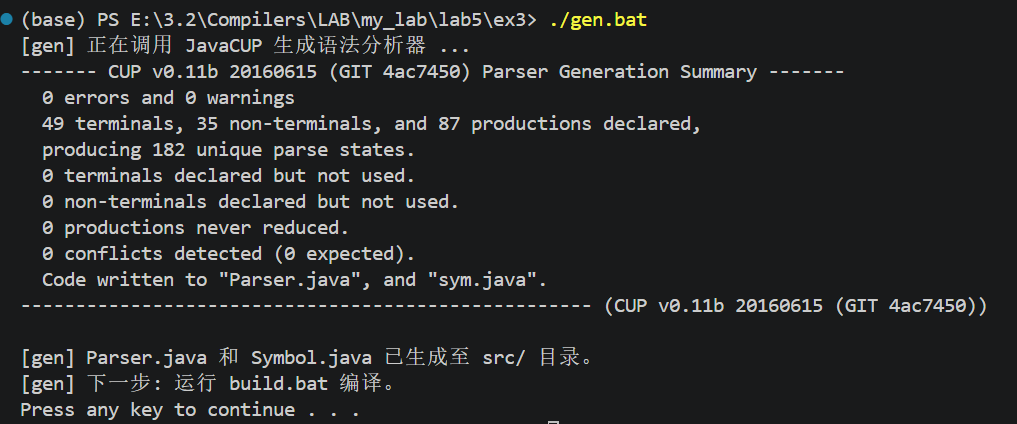
\includegraphics[width=0.9\textwidth]{img/gen_ok.png}
\caption{gen.bat 执行结果：0 错误 0 警告，生成 182 个 LALR 状态}
\label{fig:gen}
\end{figure}

\begin{figure}[H]
\centering
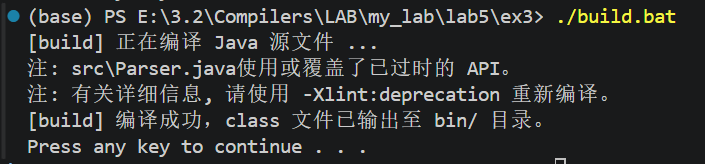
\includegraphics[width=0.9\textwidth]{img/build_ok.png}
\caption{build.bat 执行结果：所有 Java 源文件编译通过}
\label{fig:build}
\end{figure}

\section{语法分析运行结果}

图~\ref{fig:parse-term} 展示了 \texttt{run.bat} 解析 \texttt{StudentStats.obr} 的终端
输出：语法分析通过，模块 \texttt{StudentStats} 分析完成。CallGraph 统计显示 6 个过程
（CalcTotalAndAvg、ReadStudent、FindBestStudent、CheckAllPass、PrintStudent、
PrintAll）、6 个调用点和 6 条调用边。

图~\ref{fig:parse-graph} 展示了 CallGraph 弹出的可视化调用图窗口，清晰呈现了 6 个
过程节点之间的调用依赖关系。

\begin{figure}[H]
\centering
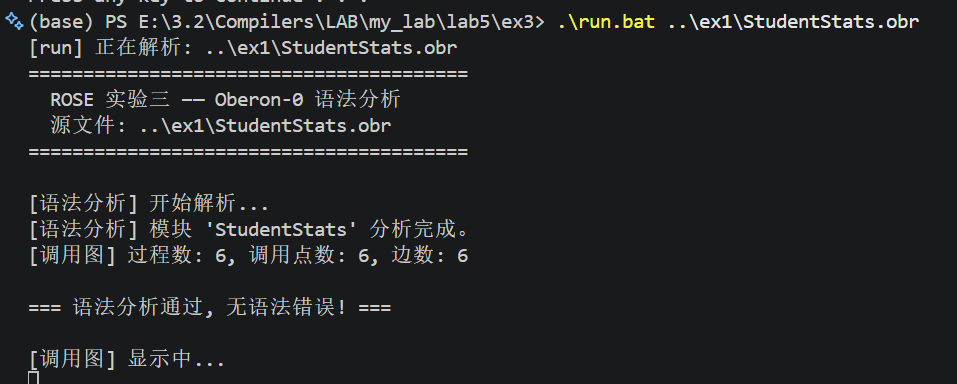
\includegraphics[width=0.9\textwidth]{img/parse_ok1.png}
\caption{StudentStats.obr 语法分析通过 —— 6 过程、6 调用点、6 边}
\label{fig:parse-term}
\end{figure}

\begin{figure}[H]
\centering
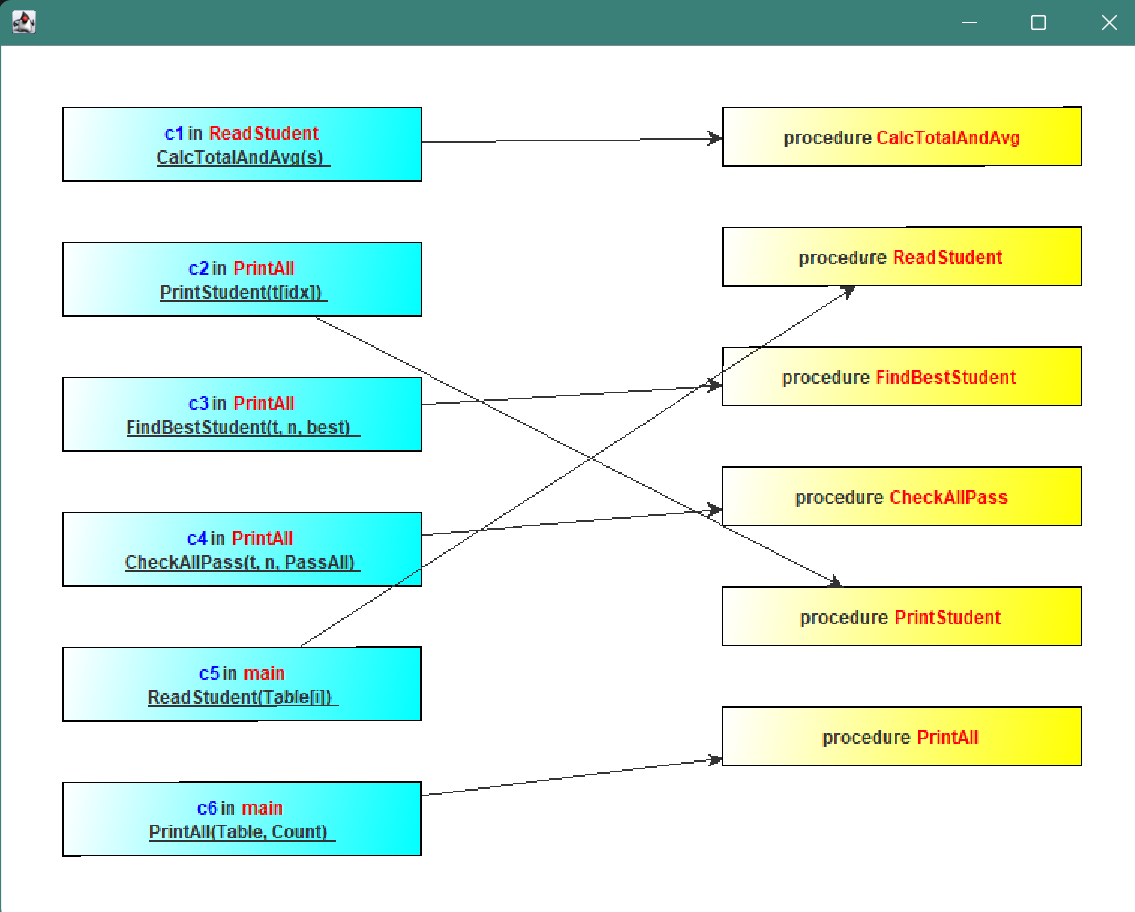
\includegraphics[width=0.9\textwidth]{img/parse_ok2.png.png}
\caption{CallGraph 调用图可视化 —— 6 个过程节点的调用依赖关系}
\label{fig:parse-graph}
\end{figure}

\section{实验心得与体会}

\begin{itemize}

\item \textbf{LL 与 LR 范式的直观对比。}
实验三（LALR 自动生成）与实验四（递归下降手写）覆盖了两种主流语法分析范式，
使我对 shift-reduce 与递归下降的决策机制差异有了具体认知。
LALR 无冲突分析表（182 状态，0 冲突）的生成过程，验证了自底向上方法对
Oberon-0 文法的完美适配。

\item \textbf{非终结符显式声明 = 编译期类型检查。}
JavaCUP 要求所有非终结符前置声明，初看冗余，实则提供了"类型检查"功能——
产生式右部与左部 \texttt{RESULT} 类型不匹配时在生成期即报警，避免了
到 javac 阶段才发现语义值传递错误。这是声明式工具链"提早暴露错误"哲学的体现。

\item \textbf{Token→sym 编码映射是最隐蔽的集成陷阱。}
JavaCUP 按声明顺序重编号终结符，与 Token.java 中手动常量完全不同。
若不通过 HashMap 桥接（49 对映射），分析器首行即报语法错误，而 Token 流调试
输出完全正确。这揭示了自动生成工具隐含约定的集成风险。

\item \textbf{语义动作嵌入语法规则 = 语法制导翻译的工程实践。}
在过程声明处调用 \texttt{graph.addProcedure()}、过程调用处调用
\texttt{graph.addEdge()}，语义动作精确嵌入在归约节点上，LALR 的归约时机
恰是所有子结构就绪的"信息汇总点"——这正是语法制导翻译（SDT）的核心思想。

\item \textbf{工具选择决定架构上限，文法规则决定质量下限。}
JavaCUP vs Bison、JavaCC vs JavaCUP 的对比表明：工具提供了分析表压缩、
类型安全、Unicode 支持等性能保障（上限），而文法编写质量决定了能否正确解析语言（下限）。

\end{itemize}
\end{document}
